\chapter{Desenvolvimento}\label{cap:CnptDsng}

\section{Escolha da frequência}\label{sec:esc_freq}
A frequência foi escolhida com base no regulamento da Anatel. O mesmo estabelece que equipamentos de radiocomunicação com faixas restritas de: 902-907,5; 915-928; 2400-2483,5; 5725-5850 MHz, assim para os cálculos iniciais foi escolhida uma frequência de 920MHz.

\section{Estudo do Obstáculo}\label{sec:est_obs}
O primeiro passado adotado foi a análise dos pontos, verificando se entre os dois existia algum obstáculo. Essa informação pode ser extraída dos mapas que foram fornecidos em anexo, como mostra a figura \ref{fig:obs_cam}.
\begin{figure}[h]
	\centering
	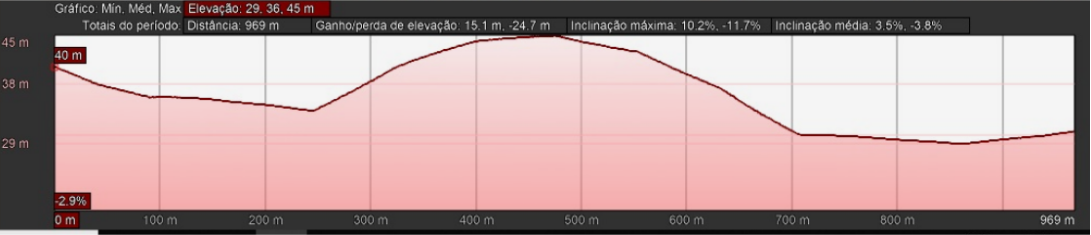
\includegraphics[width=1\textwidth]{obs_cam.png}
	\caption{Gráfico de obstáculo}
	\label{fig:obs_cam}
	%\source{Fornecido junto com os pontos}
\end{figure} 

Por meio da análise do gráfico, fica evidenciado que entre os dois pontos existe um grande obstáculo arredondado, assim sendo necessário calcular o seu raio de curvatura e a partir disso ver o quanto ele irá interferir na transmissão.
É feita uma aproximação do topo do obstáculo, utilizando uma curvatura parabólica como mostrado na figura 4 \ref{fig:obs_raio}.
\begin{figure}[h]
	\centering
	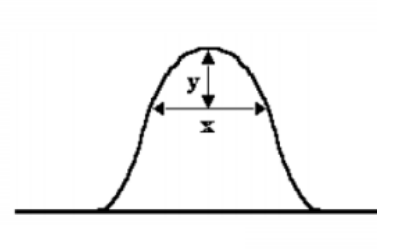
\includegraphics[width=.4\textwidth]{obs_raio.png}
	\label{fig:obs_raio}
	\caption{Curvatura parabólica utilizada para aproximação}
	%\source{Própria}
\end{figure} 

O raio $r$ da parábola será calculado o $\alpha$ que possibilita encontrar quantos decibéis de interferência o obstáculo irá causar. O cálculo do raio $r$ é feito utilizando a seguinte formula:
\begin{equation}
r = \dfrac{x^2}{8y}*10^{-3}
\end{equation}

Onde $x$ representa a distância em metros entre os dois pontos de igual nível, sendo um em cada lado do pico considerado e $y$ representa a diferença de cota entre o pico do obstáculo e a curva de nível considerada para  medida $x$.

\section{Atenuação do Obstáculo}
O cálculo do fator $\alpha$ relaciona a frequência $f$, o raio de curvatura da parábola $r$, a distância entre o vértice do obstáculo ao ponto de transmissão $d_1$ e a distância entre o vértice do obstáculo ao ponto de recepção $d_2$, ambas em \textit{Km}.
\begin{equation}
\alpha = 0,0818\dfrac{1}{\sqrt[6]{f}}\sqrt[3]{r}\sqrt{\dfrac{d_1+d_2}{d_1*d_2}}
\end{equation}

A atenuação é encontrada com o $\alpha$ e a relação entre os fatores  $H_c$ e $r_f$ por meio do gráfico 5. Onde $H_c$ representa a diferença entre ponto máximo do obstáculo e o nivelamento das antenas, enquanto $r_f$  é chamado de raio de \textit{fresnel}, sendo calculado com as mesmas distâncias $d_1$ e $d_2$. A relação é encontrada como mostrado na figura 6.

\begin{figure}[h]
	\centering
	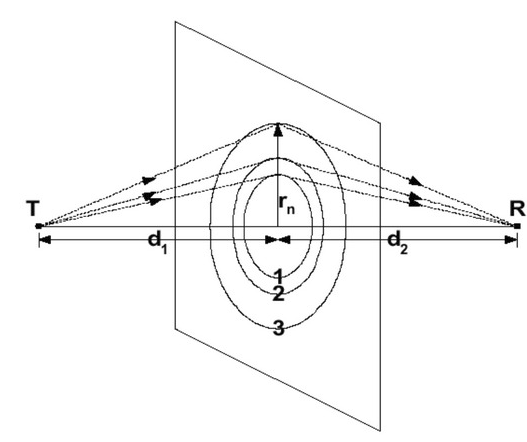
\includegraphics[width=.6\textwidth]{rf_img.png}
	\label{fig:rf_img}
	\caption{Modelo da zona de \textit{Fresnel}}
	%\source{Própria}
\end{figure}

O cálculo de $r_f$ se dá por:
\begin{equation}
r_f = \sqrt{\dfrac{n\lambda d_1 d_2}{d_1 + d_2}}
\end{equation}

\begin{figure}[h]
	\centering
	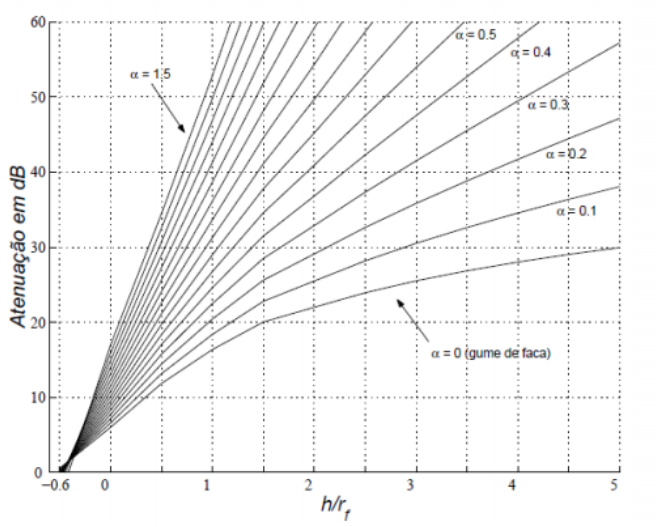
\includegraphics[width=.8\textwidth]{graf_ate.png}
	\label{fig:graf_ate}
	\caption{Gráfico de atenuação}
	%\source{Própria}
\end{figure} 

Onde o valor de $n$ foi fornecido como sendo igual a $1$ e com os valores mostrados na tabela e a análise do gráfico foi encontrado um valor de atenuação do obstáculo de $22,5dB$.

\begin{center}
	\begin{table}[]
		\begin{tabular}{|l|l|}
			\hline
			Rf    & 8,866 \\ \hline
			Hc    & 5     \\ \hline
			Hc/rf & 8,866 \\ \hline
		\end{tabular}
	\end{table}
\end{center}


\section{Atenuação no espaço livre}
O sinal também sofrerá atenuação ao ser transmitido no espaço livre, o cálculo da atenuação $L$ se deu pela seguinte equação:
\begin{equation}
L = 32,45 +20(\log_{10}(d_1+d_2) + \log_{10}f)
\end{equation}

O valor encontrado foi de $L = 91,43dB$.

\section{Escolha da Antena}
